%%%%%%%%%%%%%%%%%%%%%%%%%%%%%%%%%%%%%%%%%%%%%%%%%%%%%%%%%%%%%%%%%%%%%%%%%%%

\documentclass[a4paper,oneside,12pt]{article}
\usepackage{mystyle}

\begin{document}

\title{\Large\bf Real numbers}
\author{%%
  Minh Van Nguyen \\
  \url{mvngu@gmx.com}
}
\date{\today}
\maketitle

%%%%%%%%%%%%%%%%%%%%%%%%%%%%%%%%%%%%%%%%%%%%%%%%%%%%%%%%%%%%%%%%%%%%%%%%%%%

\section{Rational numbers}

A \emph{rational} number is a ratio of two integers.  A
rational number is also known as a fraction.  These are rational
numbers: $1/2$, $3/4$, $11/9$, and $-10/2$.  You write $5/2 \in \QQ$
to mean that $5/2$ belongs to the set of rational numbers.  The set of
all rational numbers is written as
\[
\QQ
=
\setdes{
  \frac{a}{b}
}{
  \pair{a}{b} \in \ZZ
  \text{ and }
  b \neq 0
}.
\]
This means that the set of rational numbers consists of all numbers of
the form $a/b$ such that $a$ and $b$ are integers, but $b$ cannot be
zero.  The top integer $a$ is called the \emph{numerator} and the
bottom integer $b$ is called the \emph{denominator}.  If $b = 1$, then
$a/b = a/1 = a$ and consequently any integer is also a rational
number.

\begin{exercise}
Provide an example of a rational number that is also an integer.
Explain why your number is an integer.
\end{exercise}

\ifbool{showSolution}{
\begin{solution}
The rational number $2/1$ is also an integer because it can be written
as $2/1 = 2$ and $2$ is an integer.
\end{solution}
}{}

\begin{exercise}
Give an example of a rational number that is not an integer.  Explain
why your number is not an integer.
\end{exercise}

\ifbool{showSolution}{
\begin{solution}
The ratio $1/2$ is not an integer because $1/2$ cannot be simplified
to any integer.
\end{solution}
}{}

\begin{exercise}
If $a/b$ is a rational number, why can't $b$ be zero?  Consider the
examples of $1/4$ and $1/0$.
\end{exercise}

\ifbool{showSolution}{
\begin{solution}
If in the rational number $a/b$ you have $b = 0$, then the ratio
$a / 0$ is not defined.  This means that as $b$ comes closer and
closer to zero, the value of the ratio $a/b$ does not come to a fixed
number.
\end{solution}
}{}

If $a/b$ is a rational number, there are many rational numbers that
have the same value as $a/b$.  For example, the ratio $1/2$ is the
same as the ratios $2/4$, $3/6$, and $4/8$.  The reason is that you
can write
%%
\begin{align*}
\frac{1}{2}
&=
\frac{1}{2} \times \frac{2}{2} \\[4pt]
&=
\frac{1}{2} \times \frac{3}{3} \\[4pt]
&=
\frac{1}{2} \times \frac{4}{4}.
\end{align*}
%%
In fact, if $c$ is any integer such that $c \neq 0$, then
\[
\frac{a}{b}
=
\frac{a}{b} \times \frac{c}{c}
=
\frac{ac}{bc}
\]
where the ratio $c/c$ can be simplified as $c/c = 1$.  The set $\ZZ$
of integers has an infinite number of elements because the sequence
$\seqi{1}{2}{3}$ of positive integers gets bigger and bigger and goes
on forever.  Furthermore, the sequence $\seqi{-1}{-2}{-3}$ of negative
integers gets smaller and smaller and also goes on forever.  In other
words, if $a/b$ is a rational number, then it is easy find an infinite
number of rational numbers that have the same value as $a/b$.  The
above is summarised as:

\begin{theorem}
\label{thm:infinitely_many_rationals_same_value}
If $a/b$ is a rational number such that $b \neq 0$, then there are
infinitely many rational numbers that have the same value as $a/b$.
\end{theorem}

It is because of \Theorem{thm:infinitely_many_rationals_same_value}
that you can simplify a fraction.  If a rational number $a/b$ can be
simplified, then there must be a rational number $c/d$ that has the
same value as $a/b$ but the numerator
$\absoluteValue{c} < \absoluteValue{a}$ and the denominator
$\absoluteValue{d} < \absoluteValue{b}$.  Given any number $x$, the
expression $\absoluteValue{x}$ is called the \emph{absolute value} of
$x$ and is defined as
\[
\absoluteValue{x}
=
\begin{cases}
x,  & \text{if $x \geq 0$}, \\[4pt]
-x, & \text{otherwise}.
\end{cases}
\]
For example, the absolute value of $0$ is $0$, the absolute value of
$3$ is $3$, and the absolute value of any positive number $y$ is $y$
itself.  You obtain the absolute value of a negative number by
multiplying the number by $-1$.  For example, the absolute value of
$-7$ is $\absoluteValue{-7} = -1 \times (-7) = 7$.

\begin{exercise}
Can the rational number $15 / 21$ be simplified any further?  If yes,
provide a simplified version of $15 / 21$.  If no, explain why not.
\end{exercise}

\ifbool{showSolution}{
\begin{solution}
The numerator $15$ and the denominator $21$ both have $3$ as a common
factor.  Then the rational number $15 / 21$ can be simplified as:
%%
\begin{align*}
\frac{15}{21}
&=
\frac{
  3 \times 5
}{
  3 \times 7
} \\[4pt]
&=
\frac{5}{7}.
\end{align*}
\end{solution}
}{}

\begin{exercise}
Simplify the fraction $-28 / 35$ as much as possible.
\end{exercise}

\ifbool{showSolution}{
\begin{solution}
The numerator and denominator both have $7$ as a common factor so the
fraction $-28 / 35$ can be simplified as:
%%
\begin{align*}
-\frac{28}{35}
&=
-\frac{
  7 \times 4
}{
  7 \times 5
} \\[4pt]
&=
-\frac{4}{5}.
\end{align*}
%%
Note that $\absoluteValue{-4} = 4$ and $\absoluteValue{-28} = 28$ and
so $\absoluteValue{-4} < \absoluteValue{-28}$ even though
$-28 < -4$.
\end{solution}
}{}

\begin{exercise}
Explain why the rational number $3/7$ cannot be simplified any
further.
\end{exercise}

\ifbool{showSolution}{
\begin{solution}
The only factor that $3$ and $7$ have in common is $1$.  Therefore the
rational number $3/7$ cannot be simplified any further.
\end{solution}
}{}


%%%%%%%%%%%%%%%%%%%%%%%%%%%%%%%%%%%%%%%%%%%%%%%%%%%%%%%%%%%%%%%%%%%%%%%%%%%

\section{Irrational numbers}

An \emph{irrational} number is any number that cannot be written as a
ratio of two integers.  The number $\sqrt{2}$ is an irrational number
so it cannot be an integer and cannot be written as a ratio of two
integers.  But how did you know that $\sqrt{2}$ is irrational?  How
would you prove that $\sqrt{2}$ is irrational?  The fact that
$\sqrt{2}$ is irrational can be demonstrated by using a technique
called \emph{proof by contradiction}.  The general idea of proof by
contradiction is to assume that a statement $S$ is true.  You then
work out a contradiction that results from assuming the truth of the
statement $S$.  Any statement is either true or false.  Since the
truth of the statement $S$ has led to a contradiction, it must be that
$S$ is false.

\begin{theorem}
The number $\sqrt{2}$ is irrational.
\end{theorem}

\begin{proof}
The number $\sqrt{2}$ is either rational or irrational.  To derive a
contradiction, you assume that $\sqrt{2}$ is a rational number.  Since
$\sqrt{2}$ is rational, it can be written as a ratio
%%
\begin{equation}
\label{eqn:root_2_as_ratio}
\sqrt{2}
=
\frac{a}{b}
\end{equation}
%%
where $a$ and $b$ are integers such that $b \neq 0$.  Square both
sides of \Equation{eqn:root_2_as_ratio} and you can write
\Equation{eqn:root_2_as_ratio} as
\[
(\sqrt{2})^2
=
\parenthesis*{
  \frac{a}{b}
}^2
\]
which simplifies to $2 = a^2 / b^2$.  Now solve for $a^2$ to see that
\Equation{eqn:root_2_as_ratio} can also be written as
%%
\begin{equation}
\label{eqn:root_2_a_square_is_even}
2b^2
=
a^2.
\end{equation}
%%
In other words, $a^2$ is even and $a$ must be even as well and so $a$
can be written as $a = 2k$, where $k$ is some other integer.
Substitute $a = 2k$ into \Equation{eqn:root_2_a_square_is_even} and
you get $2b^2 = (2k)^2$.  Simplify the equation $2b^2 = (2k)^2$ and
you see that \Equation{eqn:root_2_as_ratio} can also be written as
%%
\begin{equation}
\label{eqn:root_2_b_square_is_even}
b^2
=
2k^2.
\end{equation}
%%
Equation~\eqref{eqn:root_2_b_square_is_even} says that $b^2$ is even
and so $b$ is also even.  In other words, you can write $b = 2\ell$
for an integer $\ell$.  Substitute $b = 2\ell$ into
\Equation{eqn:root_2_b_square_is_even} and you have
$(2\ell)^2 = 2k^2$.  Simplify the last equation and you see that
\Equation{eqn:root_2_as_ratio} can also be written as
\[
2\ell^2
=
k^2.
\]
Solve the last equation for $2$ and you have $2 = (k / \ell)^2$.  Take
the square root of both sides of $2 = (k / \ell)^2$ and you get
$\sqrt{2} = k / \ell$.  Now use \Equation{eqn:root_2_as_ratio} to
write
\[
\sqrt{2}
=
\frac{a}{b}
=
\frac{k}{\ell}.
\]
The only way for the equation $a/b = k / \ell$ to be true is to have
$a = k$ and $b = \ell$.  Since you also have $a = 2k$, the only way
for the expression $a = k = 2k$ to be true is to have $a = 0$.
Substitute $a = 0$ into \Equation{eqn:root_2_as_ratio} and you have
$\sqrt{2} = 0 / b = 0$.  The contradiction is that $\sqrt{2} \neq 0$,
but you have shown that $\sqrt{2} = 0$.  The expressions
$\sqrt{2} \neq 0$ and $\sqrt{2} = 0$ cannot both be true at the same
time.  So something must be wrong and that something is the assumption
that $\sqrt{2}$ is a rational number.  Therefore you conclude that
$\sqrt{2}$ must be an irrational number.
\end{proof}

\begin{exercise}
Is the number $(\sqrt{2})^2$ rational or irrational?
\end{exercise}

\ifbool{showSolution}{
\begin{solution}
The number $(\sqrt{2})^2$ can be written as
%%
\begin{align*}
(\sqrt{2})^2
&=
\sqrt{2} \times \sqrt{2} \\[4pt]
&=
2.
\end{align*}
%%
Then $\sqrt{2} \times \sqrt{2} = 2$ is an integer and therefore a
rational number because you can write $2 = 2/1$.
\end{solution}
}{}

\begin{exercise}
Is the number $(\sqrt{2})^4$ rational or irrational?
\end{exercise}

\ifbool{showSolution}{
\begin{solution}
The number $(\sqrt{2})^4$ can be written as
%%
\begin{align*}
(\sqrt{2})^4
&=
(\sqrt{2})^2 \times (\sqrt{2})^2 \\[4pt]
&=
2^2 \\[4pt]
&=
4.
\end{align*}
%%
Therefore $(\sqrt{2})^4$ is a rational number.
\end{solution}
}{}

\begin{exercise}
Is the number $(\sqrt{2})^6$ rational or irrational?
\end{exercise}

\ifbool{showSolution}{
\begin{solution}
The number $(\sqrt{2})^6$ can be written as
%%
\begin{align*}
(\sqrt{2})^6
&=
(\sqrt{2})^2 \times (\sqrt{2})^2 \times (\sqrt{2})^2 \\[4pt]
&=
2^3 \\[4pt]
&=
8.
\end{align*}
%%
Therefore $(\sqrt{2})^6$ is a rational number.
\end{solution}
}{}


%%%%%%%%%%%%%%%%%%%%%%%%%%%%%%%%%%%%%%%%%%%%%%%%%%%%%%%%%%%%%%%%%%%%%%%%%%%

\section{Real numbers}

The set of \emph{real} numbers is made up of all rational and all
irrational numbers.  The set of real numbers is written as $\RR$.  For
example, the ratio $3/7$ is a real number, the square root $\sqrt{2}$
is a real number, and the integer $42$ is a real number.  Given any
number $x \in \RR$, you now have the following situation.  The number
$x$ is either rational or irrational.  If $x$ is irrational, then it
cannot be written as a ratio of two integers.  On the other hand, if
$x$ is rational, then it can be written as $x = a / b$ with $a$ and
$b$ being integers such that $b \neq 0$.  It might happen that
$b = 1$, in which case $x$ would be an integer.

\begin{exercise}
Explain why any integer is a real number.
\end{exercise}

\ifbool{showSolution}{
\begin{solution}
Any integer is also a rational number.  Since a rational number is
also a real number, it follows that any integer is also a real
number.
\end{solution}
}{}

\begin{exercise}
How can a number be represented as a picture?
\end{exercise}

\ifbool{showSolution}{
\begin{solution}
A real number can be represented as a point on the number line.
\end{solution}
}{}

\begin{exercise}
Simplify the expression
$\displaystyle{
  \frac{
    3 \times 2 + (11 - 5)
  }{
    2 \times (3 + 7)
  }
}$.
\end{exercise}

\ifbool{showSolution}{
\begin{solution}
The expression
$\displaystyle{
  \frac{
    3 \times 2 + (11 - 5)
  }{
    2 \times (3 + 7)
  }
}$
can be simplified as
%%
\begin{align*}
\frac{
  3 \times 2 + (11 - 5)
}{
  2 \times (3 + 7)
}
&=
\frac{
  3 \times 2 + 6
}{
  2 \times (3 + 7)
} \\[4pt]
&=
\frac{
  3 \times 2 + 6
}{
  2 \times 10
} \\[4pt]
&=
\frac{
  6 + 6
}{
  20
} \\[4pt]
&=
\frac{
  12
}{
  20
} \\[4pt]
&=
\frac{
  3
}{
  5
}.
\end{align*}
\end{solution}
}{}


%%%%%%%%%%%%%%%%%%%%%%%%%%%%%%%%%%%%%%%%%%%%%%%%%%%%%%%%%%%%%%%%%%%%%%%%%%%

\section*{Problem}

\begin{problem}
\item Give an example of something that can be represented as a
  rational number.
\ifbool{showSolution}{
  \begin{solution}
  The number of oranges you have eaten divided by the number of
  oranges you have altogether.
  \end{solution}
}{}

\item Present an example of something that can be represented as an
  irrational number.
\ifbool{showSolution}{
  \begin{solution}
  The \emph{unit circle} is a circle whose radius is one unit; see
  \Figure{fig:unit_circle}.  If a circle has radius $r$, then its area
  can be calculated as $\pi r^2$.  Since the radius of the unit circle
  is $r = 1$, it follows that the unit circle has an area of
  $\pi r^2 = \pi \times 1^2 = \pi$.  Therefore the area of a unit
  circle can be represented as an irrational number, i.e.~the number
  $\pi$.
  %%
  \begin{figure}[!htbp]
  \centering
  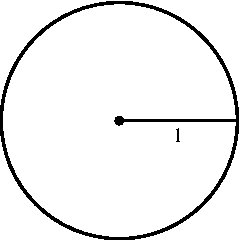
\includegraphics[scale=1]{image/02/unit-circle.pdf}
  \caption{%%
    The unit circle has a radius of one unit.  When you say
    ``one unit'' you do not care about the unit of measurement.  The
    length of the radius might be measured in terms of millimetre,
    centimetre, metre, or something else.  You are not concerned about
    these.  You only know that whatever standard of measurement is
    used, you want a value of one in terms of the scale of measurement
    that was used to measure the radius.  So the phrase ``one unit''
    can mean: one inch, one centimetre, one kilometre, etc.
  }
  \label{fig:unit_circle}
  \end{figure}
  \end{solution}
}{}

\item Provide an example of something that can be represented as a
  real number.
\ifbool{showSolution}{
  \begin{solution}
  The area of your house.
  \end{solution}
}{}

\item Simplify the expression
  \[
  E
  =
  \frac{
    3 m c^2
  }{
    (6 - 4) + 1
  }.
  \]
\ifbool{showSolution}{
  \begin{solution}
  \begin{align*}
  E
  &=
  \frac{
    3 m c^2
  }{
    (6 - 4) + 1
  } \\[4pt]
  &=
  \frac{
    3 m c^2
  }{
    2 + 1
  } \\[4pt]
  &=
  \frac{
    3 m c^2
  }{
    3
  } \\[4pt]
  &=
  m c^2.
  \end{align*}
  \end{solution}
}{}

\item Let $a$ and $b$ be integers such that $b \neq 0$.  Suppose the
  rational number $a/b$ cannot be simplified any further.
  %%
  \begin{packedenum}
  \item\label{subprob:simplify_rational_number}
    Can the rational number $\displaystyle{\frac{6a}{12b}}$ be
    simplified any further?  If yes, provide a simplified version.  If
    no, explain why not.

  \item\label{subprob:cannot_simplify_rational_number}
    Suppose $b$ is an odd integer.  Explain why the rational number
    $\displaystyle{\frac{2}{3b}}$ cannot be simplified any further.
  \end{packedenum}
\ifbool{showSolution}{
  \begin{solution}
  \solutionpart{subprob:simplify_rational_number}
  The integers $6$ and $12$ both have $6$ as a common factor.  Then
  you can simplify $\displaystyle{\frac{6a}{12b}}$ as
  %%
  \begin{align*}
  \frac{6a}{12b}
  &=
  \frac{
    6a
  }{
    6 \times 2b
  } \\[4pt]
  &=
  \frac{a}{2b}.
  \end{align*}

  \solutionpart{subprob:cannot_simplify_rational_number}
  The integers $2$ and $3$ only have $1$ as a common factor so you
  cannot simplify the ratio $2/3$ any further.  The only way for the
  expression $\displaystyle{\frac{2}{3b}}$ to be simplified any
  further is that $3b$ be even.  Since you have assumed that $b$ is
  odd, then $3b$ is also odd because the product of two odd integers
  is also an odd integer.  In other words, $2$ and $3b$ do not have
  any factor in common other than $1$.  Therefore the rational number
  $\displaystyle{\frac{2}{3b}}$ cannot be simplified any further.
  \end{solution}
}{}

\item The number $e = 2.71828\dots$ is called \emph{Euler's constant}.
  Read about $e$ on Wikipedia or search on the Internet for
  ``Euler's constant.''  Is $e$ a rational number?  Is $e$ an
  irrational number?  Is $e$ an integer?  Does $e$ belong to the set
  $\RR$ of real numbers?  Where can you find a use for the number $e$?
\ifbool{showSolution}{
  \begin{solution}
  Euler's constant $e = 2.71828\dots$ is an irrational number, which
  means that $e$ also belongs to the set of real numbers.  The number
  $e$ is used as the base of the \emph{natural logarithm},
  i.e.~logarithm to the base $e$.  The number $e$ is also used in the
  calculation of compound interest.
  \end{solution}
}{}

\item Let $n$ be an even integer such that $n \geq 0$.  Prove that the
  number $(\sqrt{2})^n$ is an integer.
\ifbool{showSolution}{
  \begin{solution}
  Since $n \geq 0$ is even, then $n$ can be written as $n = 2k$, where
  $k \geq 0$ is another integer.  Now write $(\sqrt{2})^n$ as
  %%
  \begin{align*}
  (\sqrt{2})^n
  &=
  (\sqrt{2})^{2k} \\[4pt]
  &=
  \parenthesis*{
    (\sqrt{2})^2
  }^k \\[4pt]
  &=
  2^k.
  \end{align*}
  %%
  The number $2^k$ is an integer and therefore $(\sqrt{2})^n$ is also
  an integer.
  \end{solution}
}{}
\end{problem}

\end{document}
